\chapter{Experimentos Computacionais}
\label{cap:experimentos}
Com base na abordagem metodológica apresentada no Capítulo \ref{cap:abordagem_proposta}, os experimentos computacionais foram conduzidos da seguinte maneira. Inicialmente, apresenta-se o processo de construção do conjunto de dados, conforme detalhado na Seção \ref{sec:conjunto_dados_resultados}. Em seguida, na Seção \ref{sec:modelos_parametros_resultados}, são definidos os modelos empregados na tarefa de previsão, bem como os ajustes de hiperparâmetros realizados. A Seção \ref{sec:experimentos _metricas} discute como esses modelos serão avaliados e analisados. Por fim, os resultados experimentais são apresentados na Seção \ref{sec:resultados_experimentais}.


\section{Conjunto de Dados}
\label{sec:conjunto_dados_resultados}
Para a realização dos experimentos computacionais, foram escolhidos três instrumentos financeiros: PETR3, WINFUT e WDOFUT. Amostras de cada ativo foram coletadas no período de 16/06/2021 até 16/06/2023 (2 anos), com frequências de 30 e 60 minutos. No entanto, vale ressaltar que, para o ativo WDOFUT com granularidade de 60 minutos, o intervalo considerado foi de 01/09/2021 até 01/09/2023, devido a limitações na plataforma utilizada para coleta. Essa abordagem resultou em um conjunto de dados consistente, totalizando 9156 amostras para a granularidade de 30 minutos e 4664 para a granularidade de 60 minutos. 
Posteriormente, foram criadas novas variáveis com base nos valores de \ac{OHLC}, como descrito em detalhes na Seção \ref{subsec:feature_generate}. Essas variáveis foram então escolhidas para cada conjunto de modelos de previsão, conforme explicado na Seção \ref{sec:selecao_variaveis}, onde os parâmetros $x$ e $k$ foram definidos como 8 e 4, respectivamente.

Por fim, as seis bases de dados coletadas foram categorizadas cada uma em três segmentos distintos. Dessa forma, 10\% da base de dados foi reservada para a otimização dos modelos de previsão, 70\% destinou-se ao treinamento desses modelos, e os restantes 20\% compuseram ao segmento de teste. No caso das bases de dados com granularidade de 30 minutos, essa distribuição compreendeu 916 amostras para otimização, 6409 para treinamento e 1831 para teste. Para as bases de dados com granularidade de 60 minutos, a distribuição foi de 466 amostras para otimização, 3265 para treinamento e 932 para teste. Essas alocações podem ser visualizadas nas figuras \ref{fig:PETR3_fechamento}, \ref{fig:WINFUT_fechamento} e \ref{fig:WDOFUT_fechamento}, juntamente com a tendência de cada ativo e sua faixa de variação.

\subsection{PETR3}
No contexto do ativo financeiro PETR3, o processo de construção dos \textit{datasets} (\textit{dataset1} e \textit{dataset2}) resultou em conjuntos distintos de variáveis, influenciados pelas diferentes granularidades presentes nas bases de dados. Dessa maneira, as variáveis que compõem cada conjunto de dados são as seguintes:
\begin{itemize}
	\item \textbf{\textit{dataset1} (30 minutos):} \ac{ADX} com uma janela deslizante de 14, \ac{MACD} obtido a partir do valor de fechamento com janelas deslizantes de 8 e 17 amostras, além de duas variáveis relacionadas ao \ac{ROC}. Estas referem-se à derivada do valor máximo e do fechamento, ambas com janelas deslizantes de 10 amostras.
	
	\item \textbf{\textit{dataset2} (30 minutos):} \ac{K} com uma janela deslizante de 8 amostras, \ac{TSI} obtido a partir do valor de fechamento com janelas deslizantes de 13 e 25 amostras, e mais duas variáveis relacionadas ao \ac{R} com janelas deslizantes de 14 e 21 amostras.
	
	\item \textbf{\textit{dataset1} (60 minutos):} \ac{ADX} com uma janela deslizante de 14 amostras, \ac{ROC} com janela deslizante de 10 amostras, calculado a partir do valor de fechamento, e duas variáveis relacionadas ao \ac{MACD}, ambas derivadas do valor de fechamento. Uma delas com janelas deslizantes de 12 e 26 amostras, e a outra com uma janela deslizante de 8 e 17 amostras.
	
	\item \textbf{\textit{dataset2} (60 minutos):} \ac{ROC} derivado do valor de abertura com uma janela deslizante de 12 amostras, \ac{R} com uma janela deslizante de 5 amostras, e duas variáveis associadas a \ac{K}, uma com janelas deslizantes de 8 e 10 amostras.
\end{itemize}

\begin{figure}[htbp]
	\caption{Base de dados do ativo financeiro PETR3.}
	\centering
	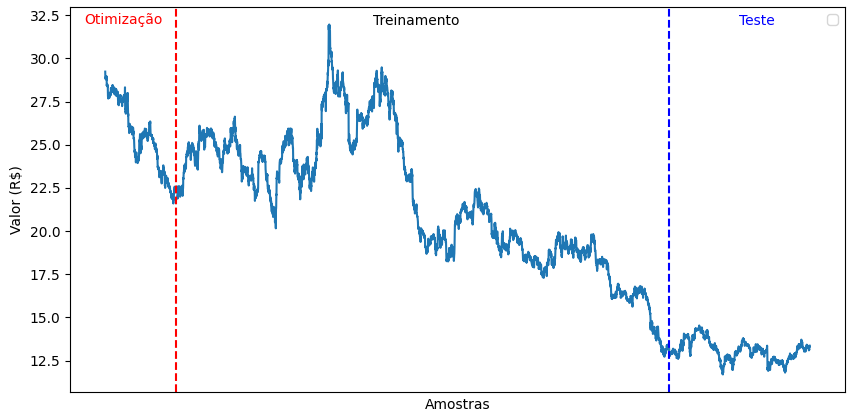
\includegraphics[width=.99\linewidth]{PETR3_fechamento.png} 
	\label{fig:PETR3_fechamento}
\end{figure}

\subsection{WINFUT}
Já no contexto do ativo financeiro WINFUT, o processo de construção dos \textit{datasets} (\textit{dataset1} e \textit{dataset2}) também resultou em conjuntos distintos de variáveis. Dessa maneira, as variáveis que compõem cada conjunto de dados são as seguintes:
\begin{itemize}
	\item \textbf{\textit{dataset1} (30 minutos):} \ac{ADX} com uma janela deslizante de 14 amostras, \ac{MACD} derivado do valor máximo com janelas deslizantes de 12 e 26 amostras, \ac{K} com uma janela deslizante de 8 amostras, e \ac{CCI} com uma janela deslizante de 18 amostras.
	
	\item \textbf{\textit{dataset2} (30 minutos):}  \ac{R} com uma janela deslizante de 5 amostras, \ac{TSI} derivado do valor de fechamento com janelas deslizantes de 13 e 25 amostras, \ac{K} com uma janela deslizante de 8 amostras, e \ac{SMA} com janela deslizante de 3 amostras.
	
	\item \textbf{\textit{dataset1} (60 minutos):} \ac{ADX} com uma janela deslizante de 14 amostras, \ac{CCI} com uma janela deslizante de 18 amostras, \ac{MACD} derivado do valor máximo com janelas deslizantes de 12 e 26 amostras, e \ac{K} com uma janela deslizante de 8 amostras.
	
	\item \textbf{\textit{dataset2} (60 minutos):} permanecem as variáveis do \textit{dataset1} de 30 minutos, com exceção da variável \ac{K}, que neste \textit{dataset} possui uma janela deslizante de 14 amostras.
\end{itemize}

\begin{figure}[htbp]
	\caption{Base de dados do ativo financeiro WINFUT.}
	\centering
	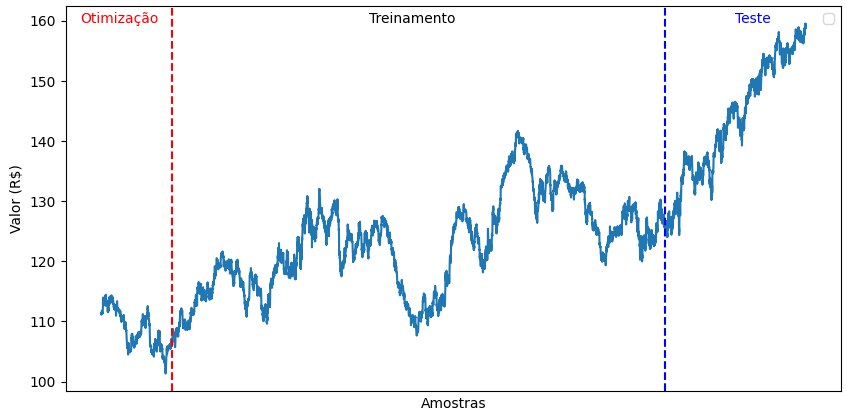
\includegraphics[width=.99\linewidth]{WINFUT_fechamento.png} 
	\label{fig:WINFUT_fechamento}
\end{figure}

\subsection{WDOFUT}
Por fim,  para o ativo financeiro WDOFUT, o processo de construção dos \textit{datasets} (\textit{dataset1} e \textit{dataset2}) também conduziu à formação de conjuntos únicos de variáveis. Desse modo, as variáveis que integram cada conjunto de dados são as seguintes:
\begin{itemize}
	\item \textbf{\textit{dataset1} (30 minutos):} \ac{ADX} com uma janela deslizante de 14 amostras, \ac{MACD} calculado a partir do valor máximo com janelas deslizantes de 12 e 26 amostras, \ac{K} com uma janela deslizante de 8 amostras, e \ac{CCI} com uma janela deslizante de 18 amostras.
	
	\item \textbf{\textit{dataset2} (30 minutos):} \ac{ADX} com uma janela deslizante de 14 amostras, \ac{ROC} obtida a partir do valor máximo com uma janela móvel de 10 amostras, e duas variáveis de \ac{MACD}. Ambas são derivadas do valor máximo, sendo uma com janelas deslizantes de 8 e 17 amostras, e a outra com janelas deslizantes de 12 e 26 amostras.
	
	\item \textbf{\textit{dataset1} (60 minutos):} \ac{ADX} com uma janela deslizante de 14 amostras, \ac{CCI} com uma janela deslizante de 18 amostras, \ac{MACD} obtido a partir do valor máximo com janelas deslizantes de 12 e 26 amostras, e \ac{K} com uma janela deslizante de 8 amostras.
	
	\item \textbf{\textit{dataset2} (60 minutos):} \ac{ADX} com uma janela deslizante de 14 amostras, \ac{ROC} calculada a partir do valor máximo com uma janela deslizante de 12 amostras, \ac{K} com uma janela deslizante de 10 amostras, e \ac{MACD} derivado do valor máximo com janelas deslizantes de 12 e 26 amostras.
\end{itemize}

\begin{figure}[htbp]
	\caption{Base de dados do ativo financeiro WDOFUT.}
	\centering
	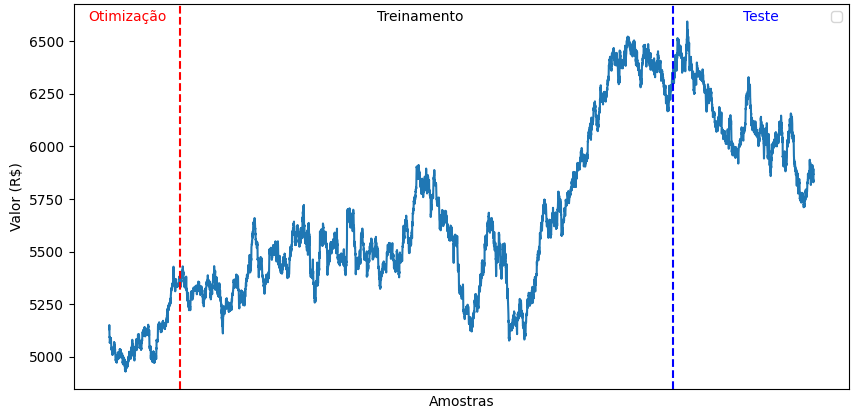
\includegraphics[width=.99\linewidth]{WDOFUT_fechamento.png} 
	\label{fig:WDOFUT_fechamento}
\end{figure}


\section{Modelos e Hiperparâmetros}
\label{sec:modelos_parametros_resultados}
Para efetivar a proposta delineada na Seção \ref{sec:previsao}, foram empregados 10 modelos distintos de previsão. No grupo de modelos estatísticos, destacam-se três escolhas específicas: \ac{ARIMA}, \ac{SARIMA}, e \ac{GARCH}. O conjunto de modelos de classificação compreende outros três: \ac{SVM}, \ac{KNN}, e \ac{LR}, enquanto o conjunto de modelos de regressão é representado por \ac{MLP}, \ac{SVR}, e \ac{RF}. Além disso, concebeu-se um modelo final, uma \ac{MLP} denominada "MLP OUT", cuja função é consolidar os resultados provenientes de cada ensemble dos três conjuntos mencionados anteriormente.
A Tabela \ref{tab:hyperparam_otmz} no Apêndice A detalha a estrutura de cada modelo de previsão, juntamente com o processo de otimização implementado e as escolhas otimizadas para cada conjunto de dados coletado. 

	
\section{Experimentos e Métricas}
\label{sec:experimentos _metricas}
As métricas de avaliação desempenham um papel crucial na análise meticulosa dos modelos propostos, sendo aplicadas a duas categorias distintas: análise de classificação e análise de recomendação de investimento.
Na fase de análise de classificação, todos os modelos definidos são considerados, uma vez que a função de transformação, que converte resultados de regressão em classificação, é aplicada uniformemente a todos os modelos de regressão. Para a avaliação desses modelos, serão utilizadas métricas essenciais, como Acurácia, \ac{F1}, e Matriz de Confusão. A Acurácia proporciona uma visão abrangente da precisão do modelo, enquanto a métrica \ac{F1} equilibra precisão e \textit{recall}, garantindo uma avaliação robusta. A Matriz de Confusão oferece uma análise mais detalhada do desempenho do modelo em diferentes categorias, proporcionando uma compreensão completa de seu comportamento em situações de classificação.

Já na análise de recomendação de investimento, todos os modelos e ensembles definidos durante o experimento são avaliados com base na estratégia delineada na Seção \ref{sec:estrategia}. Isso permite a comparação do percentual de retorno de cada modelo ao final da execução, juntamente com a quantidade de operações de compra realizadas. Importante destacar que, nessa fase, foram incorporados resultados da estratégia \textit{buy and hold} para efeitos de comparação. Essa análise final visa proporcionar \textit{insights} valiosos sobre a eficácia prática de cada abordagem na execução da estratégia proposta.

\section{Resultados Experimentais}
\label{sec:resultados_experimentais}
Nesta seção, serão detalhados os resultados provenientes dos experimentos computacionais realizados para cada conjunto de dados, acompanhados de uma análise específica destinada a cada conjunto. Essa abordagem visa oferecer uma compreensão aprofundada das conclusões derivadas da aplicação prática dos modelos em cada cenário, contribuindo para uma interpretação robusta e informada dos resultados alcançados.

\subsection{PETR3 (30 Minutos)}
Os resultados derivados da análise da base de dados PETR3, com uma granularidade de 30 minutos, são apresentados nas seções subsequentes. Inicialmente, examina-se o desempenho individual de cada modelo no contexto de classificação, seguido por uma análise detalhada no cenário de recomendação de investimento.
\subsubsection{Classificação}
Através da Tabela \ref{tab:PETR330}, observa-se que, para esta base de dados, os modelos de classificação alcançaram os melhores resultados, destacando-se em termos de acurácia e \ac{F1}, com o modelo \ac{LR} liderando. Uma consideração importante surge ao analisar a matriz de confusão do modelo \ac{ARIMA}, revelando um viés em suas classificações, comprometendo sua capacidade de identificar quedas futuras nos preços. Em síntese, o modelo de saída (\ac{MLP} OUT) da abordagem descrita na Seção \ref{sec:previsao} demonstrou um desempenho notável, assemelhando-se ao conjunto de classificação.
\LTXtable{\textwidth}{tabelas/PETR330}
\subsubsection{Recomendação de Investimento}
No âmbito da recomendação de investimento, a análise da Tabela \ref{tab:EPETR330} revela que uma elevada acurácia nem sempre se traduz em resultados financeiros vantajosos. Destaca-se que o \ac{ARIMA} alcançou o melhor desempenho, proporcionando uma variação percentual de 19,087\% a mais em relação à estratégia \textit{buy and hold}. Um resultado adicional de interesse é que a máquina de previsão proposta alcançou uma margem de 8,094\% superior à estratégia \textit{buy and hold}.
\LTXtable{\textwidth}{tabelas/EPETR330}

\subsection{PETR3 (60 Minutos)}
Os resultados provenientes da avaliação da base de dados PETR3, considerando uma granularidade de 60 minutos, estão expostos nas seções seguintes. Primeiramente, é realizada uma análise do desempenho singular de cada modelo no âmbito da classificação, seguida por uma exploração minuciosa no contexto da recomendação de investimento.
\subsubsection{Classificação}
Ao analisar a Tabela \ref{tab:PETR360}, observa-se que os modelos baseados em técnicas de regressão alcançaram o melhor resultado médio em termos de acurácia na tarefa de classificação. Como consequência, o \textit{ensemble} desse conjunto obteve os melhores resultados quando comparado com os outros \textit{ensambles}.
\LTXtable{\textwidth}{tabelas/PETR360}
\subsubsection{Recomendação de Investimento}
Quanto à recomendação de investimento, ao analisar a Tabela \ref{tab:EPETR360}, destaca-se que o \ac{KNN} apresentou os resultados mais promissores, registrando uma variação percentual de 40,508 pontos superior à estratégia \textit{buy and hold}. Esse desempenho positivo é compartilhado pelos resultados do \textit{ensemble} de classificação e do \ac{MLP} OUT, que seguem os mesmos padrões de variação.
\LTXtable{\textwidth}{tabelas/EPETR360}

\subsection{WINFUT (30 Minutos)}
Os resultados decorrentes da análise da base de dados WINFUT, considerando uma granularidade de 30 minutos, são apresentados nas seções subsequentes. Inicialmente, efetua-se uma análise do desempenho individual de cada modelo no contexto de classificação, seguida por uma exploração minuciosa na esfera da recomendação de investimento.
\subsubsection{Classificação}
Ao examinar a Tabela \ref{tab:WIN30}, percebe-se que a maioria dos resultados de classificação assume características de modelos aleatórios, com muitos deles apresentando acurácia inferior a 50\%. Nesse cenário, destaca-se que os modelos de classificação foram os que alcançaram os melhores resultados, tanto em termos de acurácia quanto de \ac{F1}. Um aspecto relevante revelado pela matriz de confusão é o viés presente no modelo ARIMA, que demonstra uma limitação em prever variações negativas.
\LTXtable{\textwidth}{tabelas/WIN30}
\subsubsection{Recomendação de Investimento}

Do ponto de vista da recomendação de investimento, ao analisar a Tabela \ref{tab:EWIN30}, destaca-se que o modelo \ac{SVR} apresentou o melhor desempenho, registrando uma variação de 9,205\% a mais no valor investido em comparação com a estratégia \textit{buy and hold}. Esse fato contribuiu para que a saída da máquina de previsão (\ac{MLP} OUT) alcançasse um resultado de 0,167\% a mais na variação do valor investido em relação à estratégia \textit{buy and hold}.
\LTXtable{\textwidth}{tabelas/EWIN30}

\subsection{WINFUT (60 Minutos)}
Os resultados provenientes da avaliação da base de dados WINFUT, com uma granularidade de 60 minutos, estão delineados nas seções que se seguem. Inicialmente, procede-se à análise do desempenho específico de cada modelo no domínio da classificação, seguida por uma exploração meticulosa no contexto da recomendação de investimento.
\subsubsection{Classificação}
Mediante a análise da Tabela \ref{tab:WIN60}, torna-se factível observar os resultados obtidos na fase de classificação, revelando desempenhos similares entre os modelos nas métricas analisadas.
\LTXtable{\textwidth}{tabelas/WIN60}
\subsubsection{Recomendação de Investimento}
Na análise do desempenho dos modelos no contexto da recomendação de investimento, a Tabela \ref{tab:EWIN60} apresenta os resultados dessa tarefa. Destaca-se que o modelo \ac{KNN} alcançou os resultados mais expressivos, superando o \textit{buy and hold} em 5.079 pontos percentuais na variação do investimento. Essa tendência positiva é compartilhada pelo \textit{ensemble} de classificação e pelo \ac{MLP} OUT, que atingem padrões semelhantes de variação.
\LTXtable{\textwidth}{tabelas/EWIN60}

\subsection{WDOFUT (30 Minutos)}
Os resultados originados da análise da base de dados WDOFUT, considerando uma granularidade de 30 minutos, estão expostos nas seções seguintes. Primeiramente, realiza-se a avaliação do desempenho particular de cada modelo no âmbito da classificação, seguida por uma exploração minuciosa no contexto da recomendação de investimento.
\subsubsection{Classificação}
Na análise apresentada na Tabela \ref{tab:WDO30}, os resultados da fase de classificação são revelados. Estes resultados sugerem características aleatórias no sistema de previsão, uma vez que todos os modelos atingiram acurácias próximas a 50\%. Um ponto adicional a ser considerado é o viés potencial no modelo \ac{ARIMA}, o que impede sua capacidade de antecipar quedas nos valores.
\LTXtable{\textwidth}{tabelas/WDO30}
\subsubsection{Recomendação de Investimento}
No âmbito da recomendação de investimento, a Tabela \ref{tab:EWDO30} destaca os resultados pertinentes a essa etapa. Observa-se que o modelo \ac{SVR} obteve os melhores resultados, superando o \textit{buy and hold} em 7,108\% na variação percentual. Outro destaque relevante é o desempenho da saída da máquina de previsão (\ac{MLP} OUT), que registrou uma diferença de 4,233\% em relação aos resultados do \textit{buy and hold} na variação percentual do valor investido.
\LTXtable{\textwidth}{tabelas/EWDO30}

\subsection{WDOFUT (60 Minutos)}
Os resultados da análise da base de dados WDOFUT, com um intervalo de 60 minutos, estão apresentados nas seções a seguir. Primeiramente, é feita uma análise do desempenho de cada modelo no contexto da classificação, seguida por uma exploração cuidadosa no contexto da recomendação de investimento.
\subsubsection{Classificação}
Os resultados da fase de classificação são apresentados na Tabela \ref{tab:WDO60}, evidenciando os melhores desempenhos em acurácia e \ac{F1} para o conjunto de modelos de classificação. Por outro lado, ao analisar a matriz de confusão, é possível identificar que o modelo \ac{ARIMA} está enviesado, perdendo, assim, a capacidade de antecipar possíveis quedas nos preços.
\LTXtable{\textwidth}{tabelas/WDO60}
\subsubsection{Recomendação de Investimento}
Na etapa de recomendação de investimentos, os resultados são apresentados na Tabela \ref{tab:EWDO60}. O modelo \ac{GARCH} apresentou o melhor desempenho na variação percentual dentre os modelos explorados, com uma diferença de -0,887\% em relação à estratégia \textit{buy and hold}. Outro resultado notável foi o da máquina de previsão (\ac{MLP} OUT), que apresentou uma diferença de -3,065\% na variação percentual em relação à estratégia \textit{buy and hold}.
\LTXtable{\textwidth}{tabelas/EWDO60}


